\chapter{Background}

The study of networks is common across several scientific disciplines, including computer science, mathematics, physics, biology, statistics and sociology. In order to effectively study and work with this data, a general understanding of the concepts of graph theory and complex networks is required. This chapter serves as jumping off point for the computer science student looking to become for familiar with these critical definitions and concepts. This chapter also introduces the fundamentals of genetic algorithms, and the concept of optimization through population based meta-heuristics.

\label{system}
\section{Elements of Graph Theory}
A \textit{Graph G} is composed of two sets, (\textit{V,E}), where \textit{V} is the set of \textit{vertices}, or \textit{nodes} and \textit{E} is the set of unordered pairs of elements of \textit{V}. If these pairs are ordered, the graph is \textit{directed}. Elements of \textit{E} are referred to as edges. An edge connects two nodes. Nodes associated with a particular edge are called \textit{endpoints}. 
\begin{figure}[!h]
	\begin{center}
		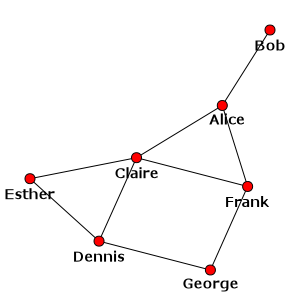
\includegraphics[scale=0.5]{images/simple_graph.png}
	\end{center}
	\caption{An undirected graph with 7 nodes and 9 edges.}
	\label{logo}
\end{figure}

A network can be visualized simply as nodes, drawn as points, connected by their corresponding edges. Note that graphs do not include self edges, called \textit{loops} or more than one edge joining the same pair of vertices. However, \textit{multigraphs} are a generalization which allow these constructs. 

A \textit{subgraph} of \textit{G = (V, E)} is denoted as \textit{$G^\prime$ = ($V^\prime$, $E^\prime$)} if \textit{$V^\prime$} $\subset$ \textit{V} and \textit{$V^\prime$} $\subset$ \textit{E}. A subgraph which contains edges such that all \textit{v}$\in$\textit{V} are endpoints is a \textit{spanning subgraph} of \textit{G}. 
A partition of a vertex set \textit{V} into two subsets \textit{S} and \textit{V $-$ S} is called a cut. The \textit{cut size} is the number of edges connecting members of \textit{S} to \textit{V $-$ S}
A \textit{path} is a finite set of edges that connect two vertices. If, for some vertices in \textit{G} no path exists, \textit{G} is a \textit{disconnected} graph.

The number of vertices and edges of a graph are indicated with \textit{n} and \textit{m}. \textit{n} is the order of a graph, and \textit{m} is the size. The maximum size of a graph if order \textit{n} is $n(n-1)/2$, the number of unordered pairs of vertices. If \textit{G} is of maximum size, each vertex having an edge to every other, it is a \textit{complete graph}. 
A fully connected subgraph is called a \textit{clique}. Endpoints are referred to as \textit{neighbors}, or \textit{adjacent nodes}. The the set of neighbors of vertex \textit{v} is the \textit{neighborhood}, indicated as \textit{$\Gamma(v)$}. $|\Gamma(v)|$, the number of neighbors of \textit{v}, is the degree of \textit{v}, $k_v$. The \textit{degree sequence} of $G$ is the list of degrees for each vertex of $G$, $k_{v1}, k_{v2},..., k_{vn}$. 
A regular graph is one whose degree sequence contains only copies of a single integer. Directed graphs distinguish between the \textit{indegree} and \textit{outdegree}, the number of edges ending at \textit{v}, and beginning at \textit{v} respectively. While in this paper we limit experiments to unweighted graphs, it is important to understand the extension of edges from being counted as binary entities, to ones with real values. These edge values are called \textit{weights}. The analog to degree of $v$ in these graphs is \textit{strength}, the sum of edge weights adjacent to $v$.

The \textit{internal degree} and \textit{external degree}, $k^{int}_i$ and $k^{ext}_i$, with respect to node $i$ being a member of subgraph $C\subset G$, are the sum of edges connecting $i$ to nodes in $C$ and not contained in $C$ respectively. 
Another useful property of vertices is \textit{clustering} \cite{Watts1998}, or \textit{transitivity} to avoid confusion when dealing with structural clusters. $C_v$, the transitivity of $v$, is the ratio of edges joining pairs of nodes in $\Gamma(v)$, to the total possible number of edges between nodes in $\Gamma(v)$. If we consider the neighborhood of $v$ as a subgraph $S$, the transitivity is given as: $$\dfrac{S_m}{k_v(k_v-1)/2}$$

A common mathmatical procedure to apply to graphs is a \textit{random walk}. As the name implies, it is  randomly generated set of steps along a path. Given a node, selected as the starting point, each step is making the transition from the current node $i$, to the next node $j$, given that $j\in\Gamma{i}$ with the probability $\frac{1}{k_i}$. Random walks have varied applications to problems in graph theory, and are a common feature of community detection methods \cite{Pons2006}.


\pagebreak
\subsection{The Adjacency Matrix}
When dealing with graphs, one of the most effective ways to represent their structure, or \textit{topology}, is an \textit{adjacency matrix}. For a binary graph $G$, its adjacency matrix is an $n\times n$ matrix $A$. Where nodes $i$ and $j$ share an edge, $A_{ij}$ is 1, and otherwise 0. This matrix is symmetric in the case of undirected graphs. The sum of the $i$-th row of $A$ is the degree of node $i$.
When The graph is weighted, it is indicated as $W$, where connected the element $W_{ij}$ is the weight of adjacent nodes $i$ and $j$.

\section{Complex Networks}
The great numbers of applications of graph theory have made it one of the foundational concepts in several fields. With this abundance of interest, a shift has occurred away from understanding local properties in small graphs, to understanding the larger statistical properties of large systems. 


\begin{figure}[!h]
	\begin{center}
		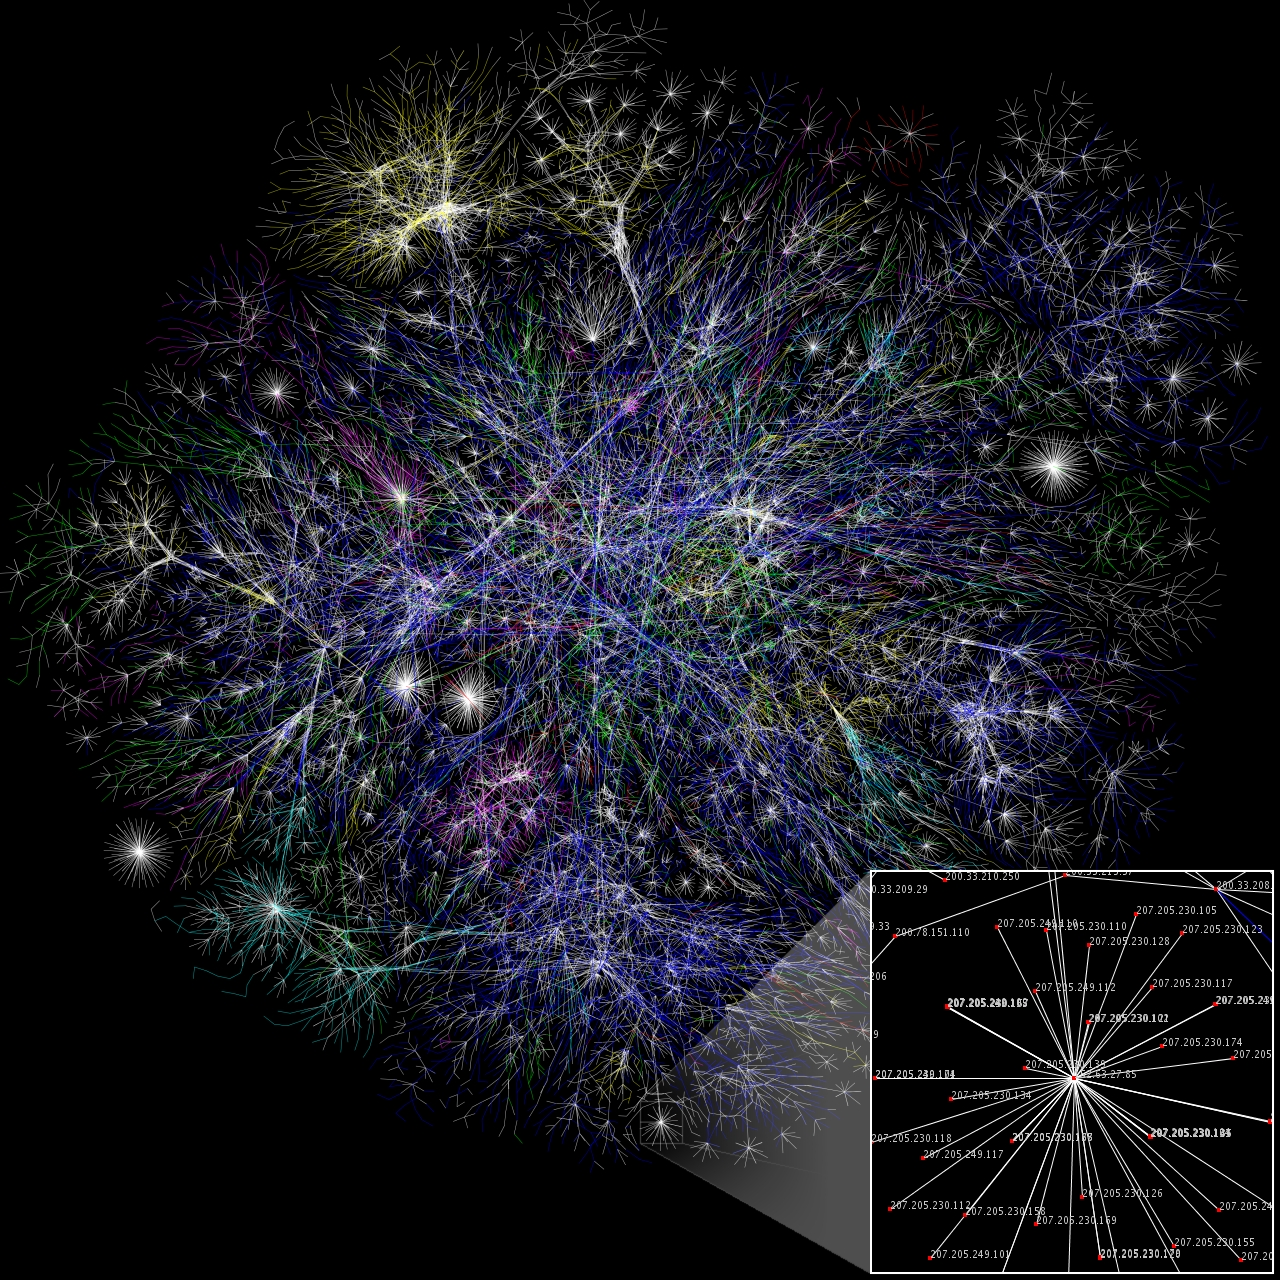
\includegraphics[scale=0.2]{images/Internet_map_1024.jpg}
	\end{center}
	\caption{A section of the Internet, as represented by the Opte Project in 2005.}
	\label{logo}
\end{figure}

\subsection{}

\section{Community Detection In Graphs}
When visualizing real world networks, it is common to see some structure in the noise. In social graphs, these may be close friend groups. In collaboration networks, groups of researchers may interact closely to those in related fields, but rarely with those more removed from their areas of interest. These \textit{communities} can offer a better understanding to how the network is organized, and how these modules may or may not interact. It gives researchers a way to identify smaller sections of interest in networks for closer study. It offers a method to classify nodes based on their role, or relationship to the structure.
\begin{figure}[!h]
	\begin{center}
		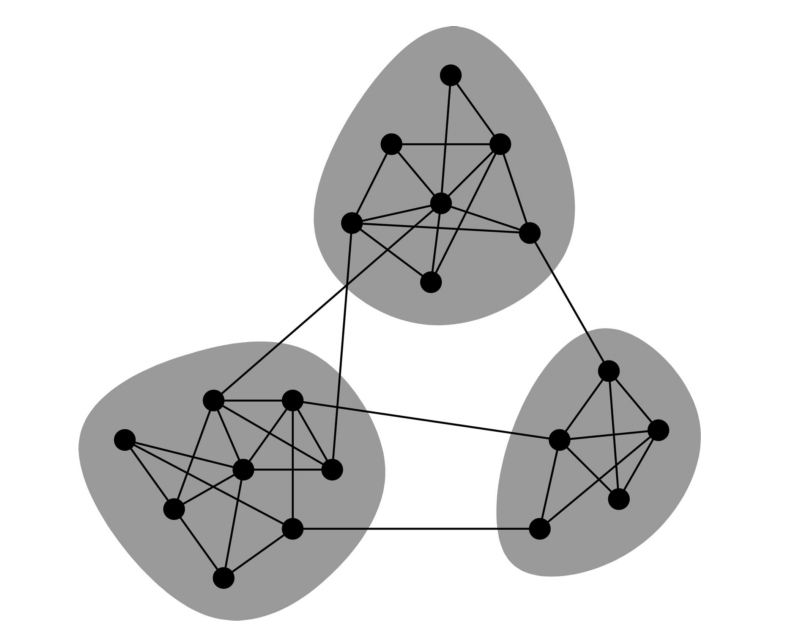
\includegraphics[scale=0.7]{images/communities.png}
	\end{center}
	\caption{Each shaded area of the graph is a community component}
	\label{logo}
\end{figure}


Community detection is not a well defined problem, however. A blanket definition for what is a good or bad structure is not offered. Because of this, it is difficult to evaluate and compare methods. A graph being used in the field of communications planning will be completely different in its properties to a network of protein-protein interactions.

The identification and study of community structure has 3 major advantages \cite{Lancichinetti2010}. First, it shows the organization of the graph at a courser level, as if it were compressed. This understanding can allow for better insights into how the network was built, and how it may continue to evolve. Secondly, 

\subsection{Defining Communities}

The problem of community detection is not well defined.

%% embeddedness perspective
Embeddedness $\xi_i$ is the ratio $\frac{k^{int}_i}{k_i}$. A higher value of $\xi_i$ indicates that $i$ is more closely associated with its community.   


\subsection{Complexity}


\subsection{Related Problems}




\section{Genetic Algorithms}
The early decades of the study of computer science saw many computational strategies inspired by the natural world. In the 1950s and 1960s, a popular idea was to use the principals of Darwinian evolution to evolve a a set of candidate solutions to a problem, by performing some set of operations taken from natural processes. These ideas grew and became the field of \textit{evolutionary computation}. Genetic algorithms, invented and developed by John Holland \cite{holland1975adaptation} are an abstraction of biological evolution, in the constraints of a genetic framework. 

%% early GA application to large data 
\cite{Ding2007}

\subsection{Motivation}


\subsection{Biological Terms}
As they are biologically inspired, it follows that the components of a GA are written about using corresponding biological terms, although the constructs they refer to in the computational context are much simpler than their living counterparts.

Each and every organism is composed of cells. Every cell contains a set of genetic materials, \textit{chromosomes}, which are the blueprint for the characteristics of the organism. A chromosome can be divided into genes, codes of DNA or RNA defining a function of a molecule. These manifest as traits such as blood type, hair and eye color, strength or intelligence. Depending on its traits, an individual may be more likely to generate offspring. The ability for life to reproduce itself and create future, surviving and multiplying generations is a generalization of what makes a species successful. However, in the natural world, populations are diverse. As reproduce via sexual reproduction, a mixing of genetic material of both parents takes place, and occasionally, an external factor will change the coding of a gene or genes, resulting in a \textit{mutation}.  

\subsection{The Population}


\subsection{Operators}


\subsubsection{Selection}


\subsubsection{Crossover}


\subsubsection{Mutation}



\begin{figure}[!htb]
	\begin{center}
		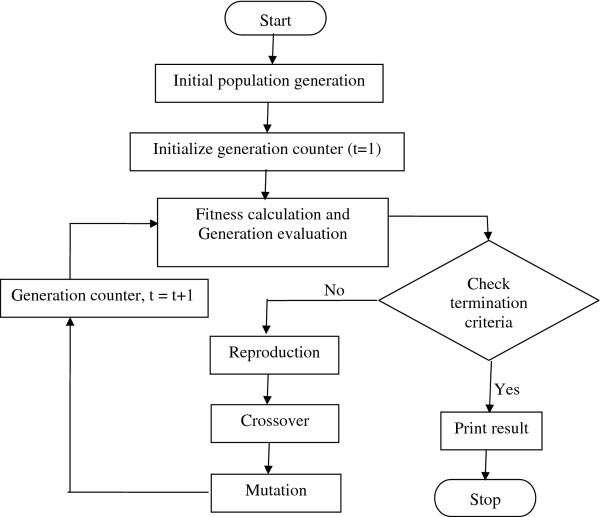
\includegraphics[scale=.75]{images/genetic_typical.png}
	\end{center}
	\caption{The flow of a typical genetic algorithm.}
	\label{logo}
\end{figure}

\begin{table}[b]
\caption{Locus Decoding Algorithm}
\label{algorithmX}
\begin{verbatim}
Decode() {
    current_c = 1
    cluster_assign = int[N]
    prv = int[N]
    for(i in 1 to N){
        cluster_assign = -1
    }
    for(i in 1 to N){
        ctr = 1
        if(cluster_assign[i] == -1){
            cluster_assign[1] = current_c
            neighbour = locus[i]
        }
    }
}
\end{verbatim}
\end{table}

